\documentclass[journal,12pt,twocolumn]{IEEEtran}
%
\usepackage{setspace}
\usepackage{gensymb}
\usepackage{xcolor}
\usepackage{caption}
%\usepackage{subcaption}
%\doublespacing
\singlespacing

%\usepackage{graphicx}
%\usepackage{amssymb}
%\usepackage{relsize}
\usepackage[cmex10]{amsmath}
\usepackage{mathtools}
%\usepackage{amsthm}
%\interdisplaylinepenalty=2500
%\savesymbol{iint}
%\usepackage{txfonts}
%\restoresymbol{TXF}{iint}
%\usepackage{wasysym}
\usepackage{hyperref}
\usepackage{amsthm}
\usepackage{mathrsfs}
\usepackage{txfonts}
\usepackage{stfloats}
\usepackage{cite}
\usepackage{cases}
\usepackage{subfig}
%\usepackage{xtab}
\usepackage{longtable}
\usepackage{multirow}
%\usepackage{algorithm}
%\usepackage{algpseudocode}
%\usepackage{enumerate}
\usepackage{enumitem}
\usepackage{mathtools}
%\usepackage{iithtlc}
%\usepackage[framemethod=tikz]{mdframed}
\usepackage{listings}
\newcommand{\myvec}[1]{\ensuremath{\begin{pmatrix}#1\end{pmatrix}}}
\newcommand{\solution}{\noindent \textbf{Solution: }}
\providecommand{\pr}[1]{\ensuremath{\Pr\left(#1\right)}}
\providecommand{\brak}[1]{\ensuremath{\left(#1\right)}}
\providecommand{\cbrak}[1]{\ensuremath{\left\{#1\right\}}}
\providecommand{\sbrak}[1]{\ensuremath{\left[#1\right]}}
\providecommand{\mean}[1]{E\left[ #1 \right]}
\providecommand{\var}[1]{\mathrm{Var}\left[ #1 \right]}
\providecommand{\der}[1]{\mathrm{d} #1}
\providecommand{\gauss}[2]{\mathcal{N}\ensuremath{\left(#1,#2\right)}}
\providecommand{\mbf}{\mathbf}
\providecommand{\abs}[1]{\left\vert#1\right\vert}
\providecommand{\norm}[1]{\left\lVert#1\right\rVert}
\providecommand{\z}[1]{{\mathcal{Z}}\{#1\}}
\providecommand{\ztrans}{\overset{\mathcal{Z}}{ \rightleftharpoons}}

\providecommand{\parder}[2]{\frac{\partial}{\partial #2} \brak{#1}}

\let\StandardTheFigure\thefigure
\let\vec\mathbf

\numberwithin{equation}{section}
\renewcommand{\thefigure}{\theenumi}
\renewcommand\thesection{\arabic{section}}

\newcommand{\myvec}[1]{\ensuremath{\begin{pmatrix}#1\end{pmatrix}}}
\newcommand{\mymat}[1]{\ensuremath{\begin{bmatrix}#1\end{bmatrix}}}
\newcommand{\mydet}[1]{\ensuremath{\begin{vmatrix}#1\end{vmatrix}}}
\newcommand{\define}{\stackrel{\triangle}{=}}

\DeclareMathOperator*{\argmin}{arg\,min}
\DeclareMathOperator*{\argmax}{arg\,max}

\makeatletter
\def\pld@CF@loop#1+{%
    \ifx\relax#1\else
        \begingroup
          \pld@AccuSetX11%
          \def\pld@frac{{}{}}\let\pld@symbols\@empty\let\pld@vars\@empty
          \pld@false
          #1%
          \let\pld@temp\@empty
          \pld@AccuIfOne{}{\pld@AccuGet\pld@temp
                            \edef\pld@temp{\noexpand\pld@R\pld@temp}}%
           \pld@if \pld@Extend\pld@temp{\expandafter\pld@F\pld@frac}\fi
           \expandafter\pld@CF@loop@\pld@symbols\relax\@empty
           \expandafter\pld@CF@loop@\pld@vars\relax\@empty
           \ifx\@empty\pld@temp
               \def\pld@temp{\pld@R11}%
           \fi
          \global\let\@gtempa\pld@temp
        \endgroup
        \ifx\@empty\@gtempa\else
            \pld@ExtendPoly\pld@tempoly\@gtempa
        \fi
        \expandafter\pld@CF@loop
    \fi}
\def\pld@CMAddToTempoly{%
    \pld@AccuGet\pld@temp\edef\pld@temp{\noexpand\pld@R\pld@temp}%
    \pld@CondenseMonomials\pld@false\pld@symbols
    \ifx\pld@symbols\@empty \else
        \pld@ExtendPoly\pld@temp\pld@symbols
    \fi
    \ifx\pld@temp\@empty \else
        \pld@if
            \expandafter\pld@IfSum\expandafter{\pld@temp}%
                {\expandafter\def\expandafter\pld@temp\expandafter
                    {\expandafter\pld@F\expandafter{\pld@temp}{}}}%
                {}%
        \fi
        \pld@ExtendPoly\pld@tempoly\pld@temp
        \pld@Extend\pld@tempoly{\pld@monom}%
    \fi}
\makeatother

\lstset {
	frame=single, 
	breaklines=true,
	columns=fullflexible,
	autogobble=true
}             

%\usepackage{stmaryrd}


%\usepackage{wasysym}
%\newcounter{MYtempeqncnt}
\DeclareMathOperator*{\Res}{Res}
%\renewcommand{\baselinestretch}{2}
\renewcommand\thesection{\arabic{section}}
\renewcommand\thesubsection{\thesection.\arabic{subsection}}
\renewcommand\thesubsubsection{\thesubsection.\arabic{subsubsection}}

\renewcommand\thesectiondis{\arabic{section}}
\renewcommand\thesubsectiondis{\thesectiondis.\arabic{subsection}}
\renewcommand\thesubsubsectiondis{\thesubsectiondis.\arabic{subsubsection}}

%\renewcommand{\labelenumi}{\textbf{\theenumi}}
%\renewcommand{\theenumi}{P.\arabic{enumi}}

% correct bad hyphenation here
\hyphenation{op-tical net-works semi-conduc-tor}

\lstset{
language=Python,
frame=single, 
breaklines=true,
columns=fullflexible
}



\begin{document}
%

\theoremstyle{definition}
\newtheorem{theorem}{Theorem}[section]
\newtheorem{problem}{Problem}
\newtheorem{proposition}{Proposition}[section]
\newtheorem{lemma}{Lemma}[section]
\newtheorem{corollary}[theorem]{Corollary}
\newtheorem{example}{Example}[section]
\newtheorem{definition}{Definition}[section]
%\newtheorem{algorithm}{Algorithm}[section]
%\newtheorem{cor}{Corollary}
\newcommand{\BEQA}{\begin{eqnarray}}
\newcommand{\EEQA}{\end{eqnarray}}
\newcommand{\define}{\stackrel{\triangle}{=}}
\bibliographystyle{IEEEtran}
%\bibliographystyle{ieeetr}
\providecommand{\nCr}[2]{\,^{#1}C_{#2}} % nCr
\providecommand{\nPr}[2]{\,^{#1}P_{#2}} % nPr
\providecommand{\mbf}{\mathbf}
\providecommand{\pr}[1]{\ensuremath{\Pr\left(#1\right)}}
\providecommand{\qfunc}[1]{\ensuremath{Q\left(#1\right)}}
\providecommand{\sbrak}[1]{\ensuremath{{}\left[#1\right]}}
\providecommand{\lsbrak}[1]{\ensuremath{{}\left[#1\right.}}
\providecommand{\rsbrak}[1]{\ensuremath{{}\left.#1\right]}}
\providecommand{\brak}[1]{\ensuremath{\left(#1\right)}}
\providecommand{\lbrak}[1]{\ensuremath{\left(#1\right.}}
\providecommand{\rbrak}[1]{\ensuremath{\left.#1\right)}}
\providecommand{\cbrak}[1]{\ensuremath{\left\{#1\right\}}}
\providecommand{\lcbrak}[1]{\ensuremath{\left\{#1\right.}}
\providecommand{\rcbrak}[1]{\ensuremath{\left.#1\right\}}}
\theoremstyle{remark}
\newtheorem{rem}{Remark}
\newcommand{\sgn}{\mathop{\mathrm{sgn}}}
\providecommand{\abs}[1]{\left\vert#1\right\vert}
\providecommand{\res}[1]{\Res\displaylimits_{#1}} 
\providecommand{\norm}[1]{\lVert#1\rVert}
\providecommand{\mtx}[1]{\mathbf{#1}}
\providecommand{\mean}[1]{E\left[ #1 \right]}
\providecommand{\fourier}{\overset{\mathcal{F}}{ \rightleftharpoons}}
\providecommand{\ztrans}{\overset{\mathcal{Z}}{ \rightleftharpoons}}
%\providecommand{\hilbert}{\overset{\mathcal{H}}{ \rightleftharpoons}}
\providecommand{\system}{\overset{\mathcal{H}}{ \longleftrightarrow}}
	%\newcommand{\solution}[2]{\textbf{Solution:}{#1}}
\newcommand{\solution}{\noindent \textbf{Solution: }}
\providecommand{\dec}[2]{\ensuremath{\overset{#1}{\underset{#2}{\gtrless}}}}
\numberwithin{equation}{section}
%\numberwithin{equation}{subsection}
%\numberwithin{problem}{subsection}
%\numberwithin{definition}{subsection}
\makeatletter
\@addtoreset{figure}{problem}
\makeatother
\let\StandardTheFigure\thefigure
%\renewcommand{\thefigure}{\theproblem.\arabic{figure}}
\renewcommand{\thefigure}{\theproblem}
%\numberwithin{figure}{subsection}
\def\putbox#1#2#3{\makebox[0in][l]{\makebox[#1][l]{}\raisebox{\baselineskip}[0in][0in]{\raisebox{#2}[0in][0in]{#3}}}}
     \def\rightbox#1{\makebox[0in][r]{#1}}
     \def\centbox#1{\makebox[0in]{#1}}
     \def\topbox#1{\raisebox{-\baselineskip}[0in][0in]{#1}}
     \def\midbox#1{\raisebox{-0.5\baselineskip}[0in][0in]{#1}}
\vspace{3cm}
\title{ 
%\logo{
Digital Signal Processing
%}
%	\logo{Octave for Math Computing }
}
%\title{
%	\logo{Matrix Analysis through Octave}{\begin{center}\includegraphics[scale=.24]{tlc}\end{center}}{}{HAMDSP}
%}
% paper title
% can use linebreaks \\ within to get better formatting as desired
%\title{Matrix Analysis through Octave}
%
%
% author names and IEEE memberships
% note positions of commas and nonbreaking spaces ( ~ ) LaTeX will not break
% a structure at a ~ so this keeps an author's name from being broken across
% two lines.
% use \thanks{} to gain access to the first footnote area
% a separate \thanks must be used for each paragraph as LaTeX2e's \thanks
% was not built to handle multiple paragraphs
%
\author{ Shreyas Wankhede

}
% note the % following the last \IEEEmembership and also \thanks - 
% these prevent an unwanted space from occurring between the last author name
% and the end of the author line. i.e., if you had this:
% 
% \author{....lastname \thanks{...} \thanks{...} }
%                     ^------------^------------^----Do not want these spaces!
%
% a space would be appended to the last name and could cause every name on that
% line to be shifted left slightly. This is one of those "LaTeX things". For
% instance, "\textbf{A} \textbf{B}" will typeset as "A B" not "AB". To get
% "AB" then you have to do: "\textbf{A}\textbf{B}"
% \thanks is no different in this regard, so shield the last } of each \thanks
% that ends a line with a % and do not let a space in before the next \thanks.
% Spaces after \IEEEmembership other than the last one are OK (and needed) as
% you are supposed to have spaces between the names. For what it is worth,
% this is a minor point as most people would not even notice if the said evil
% space somehow managed to creep in.
% The paper headers
%\markboth{Journal of \LaTeX\ Class Files,~Vol.~6, No.~1, January~2007}%
%{Shell \MakeLowercase{\textit{et al.}}: Bare Demo of IEEEtran.cls for Journals}
% The only time the second header will appear is for the odd numbered pages
% after the title page when using the twoside option.
% 
% *** Note that you probably will NOT want to include the author's ***
% *** name in the headers of peer review papers.                   ***
% You can use \ifCLASSOPTIONpeerreview for conditional compilation here if
% you desire.
% If you want to put a publisher's ID mark on the page you can do it like
% this:
%\IEEEpubid{0000--0000/00\$00.00~\copyright~2007 IEEE}
% Remember, if you use this you must call \IEEEpubidadjcol in the second
% column for its text to clear the IEEEpubid mark.
% make the title area
\maketitle
%\newpage
\tableofcontents
%\renewcommand{\thefigure}{\thesection.\theenumi}
%\renewcommand{\thetable}{\thesection.\theenumi}
\renewcommand{\thefigure}{\theenumi}
\renewcommand{\thetable}{\theenumi}
%\renewcommand{\theequation}{\thesection}
\bigskip
\begin{abstract}
This manual provides a simple introduction to digital signal processing.
\end{abstract}
\section{Software Installation}
Run the following commands
\begin{lstlisting}
sudo apt-get update
sudo apt-get install libffi-dev libsndfile1 python3-scipy  python3-numpy python3-matplotlib 
sudo pip install cffi pysoundfile 
\end{lstlisting}
\section{Digital Filter}
\begin{enumerate}[label=\thesection.\arabic*
,ref=\thesection.\theenumi]
\item
\label{prob:input}
Download the sound file from  
\begin{lstlisting}
	https://github.com/shreyaswankhede12/EE3900/blob/master/Assignment%201/sound/Sound_Noise.wav
\end{lstlisting}
%\href{http://tlc.iith.ac.in/img/sound/Sound_Noise.wav}{\url{http://tlc.iith.ac.in/img/sound/Sound_Noise.wav}}  
%in the link given below.
%\linebreak
\item
\label{prob:spectrogram}
You will find a spectrogram at \href{https://academo.org/demos/spectrum-analyzer}{\url{https://academo.org/demos/spectrum-analyzer}}. 
%\end{problem}
%%
%
%%\onecolumn
%%\input{./figs/fir}
%\begin{problem}
Upload the sound file that you downloaded in Problem \ref{prob:input} in the spectrogram  and play.  Observe the spectrogram. What do you find?
\\
%
\solution There are a lot of yellow lines between 440 Hz to 5.1 KHz.  These represent the synthesizer key tones. Also, the key strokes
are audible along with background noise.
% By observing spectrogram, it clearly shows that tonal frequency is under 4kHz. And above 4kHz only noise is present.
\item
\label{prob:output}
Write the python code for removal of out of band noise and execute the code.
\\
\solution
\begin{lstlisting}
	https://github.com/shreyaswankhede12/EE3900/blob/master/Assignment%201/codes/qs%202/Cancel_noise.py
\end{lstlisting}
% \lstinputlisting{codes/Cancel_noise.py}
%\begin{figure}[h]
%\centering
%\includegraphics[width=\columnwidth]{enc_block_diag.png}
%\caption{}
%\label{fig:convolution encoder}
%\end{figure}
%\input{block_enc}
\item
The output of the python script in Problem \ref{prob:output} is the audio file Sound\_With\_ReducedNoise.wav. Play the file in the spectrogram in Problem \ref{prob:spectrogram}. What do you observe?
\\
\solution The key strokes as well as background noise is subdued in the audio.  Also,  the signal is blank for frequencies above 5.1 kHz.
\end{enumerate}
\section{Difference Equation}
\begin{enumerate}[label=\thesection.\arabic*,ref=\thesection.\theenumi]
\item Let
\begin{equation}
x(n) = \cbrak{\underset{\uparrow}{1},2,3,4,2,1}
\end{equation}
Sketch $x(n)$.
\begin{figure}[!ht]
	\begin{center}
	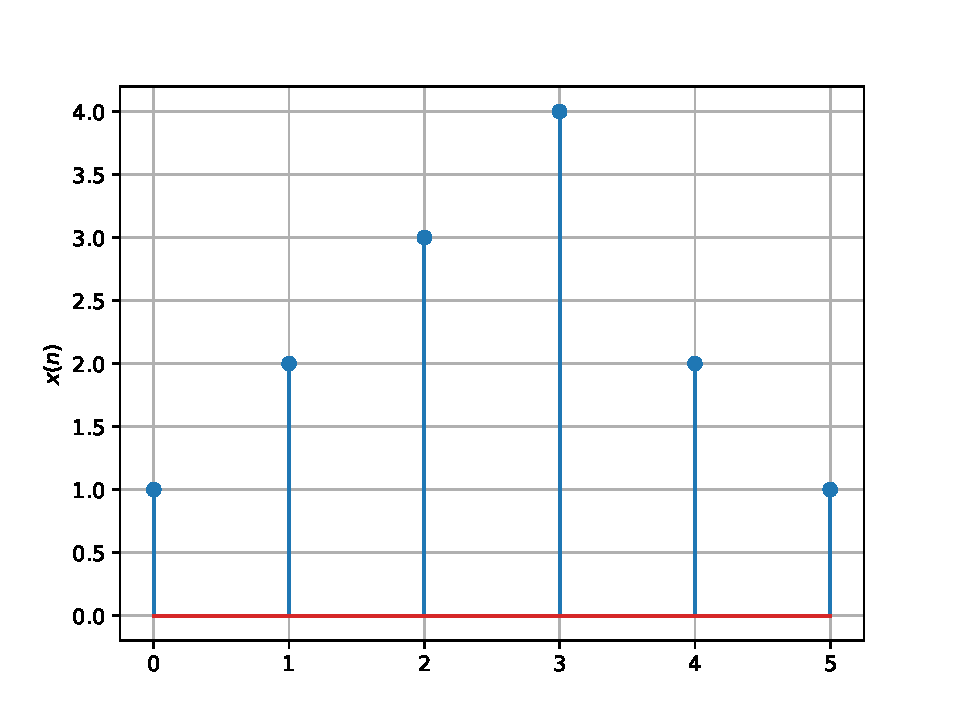
\includegraphics[width=\columnwidth]{figs/3.1 xn}
	\end{center}
	\captionof{figure}{}
	\label{fig:xn}	
	\end{figure}
\item Let
\begin{multline}
\label{eq:iir_filter}
y(n) + \frac{1}{2}y(n-1) = x(n) + x(n-2), 
\\
 y(n) = 0, n < 0
\end{multline}
Sketch $y(n)$.
\begin{figure}[!ht]
	\begin{center}
	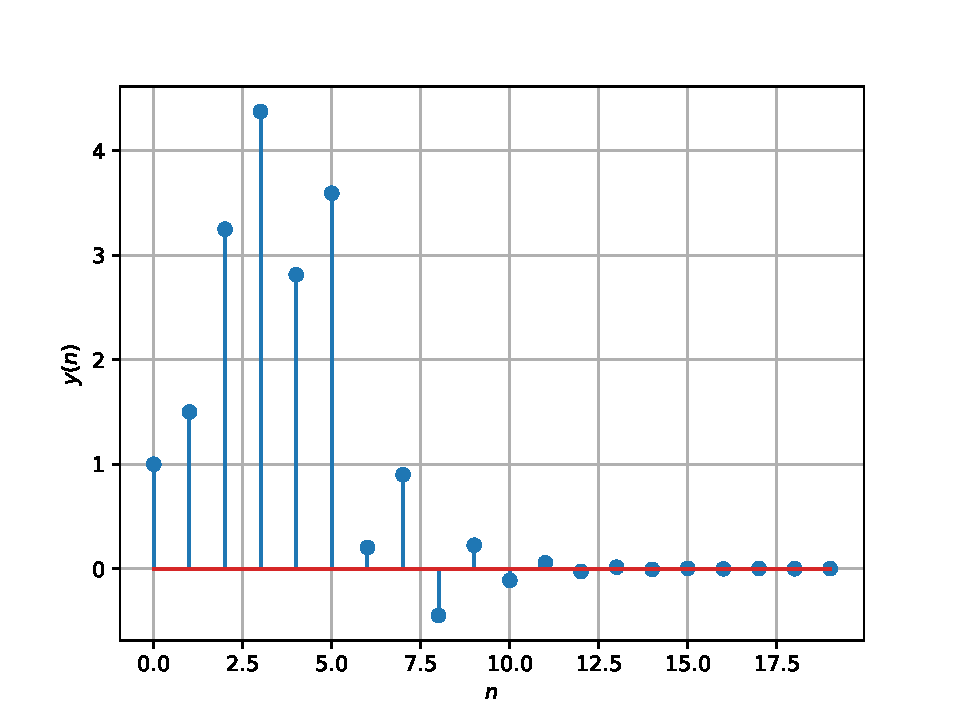
\includegraphics[width=\columnwidth]{figs/3.2 yn}
	\end{center}
	\captionof{figure}{}
	\label{fig:xnyn}	
	\end{figure}
\\
\solution The following code yields Fig. \ref{fig:xnyn}.
\begin{lstlisting}
	https://github.com/shreyaswankhede12/EE3900/blob/master/Assignment%201/codes/qs%203/xn.py\\
	https://github.com/shreyaswankhede12/EE3900/blob/master/Assignment%201/codes/qs%203/yn.py
\end{lstlisting}
\item Repeat the above exercise using a C code.
\solution Run the following C code.
\begin{lstlisting}
	https://github.com/shreyaswankhede12/EE3900/blob/master/Assignment%201/codes/qs%203/xn_yn.C
\end{lstlisting}
\end{enumerate}
\section{$Z$-transform}
\begin{enumerate}[label=\thesection.\arabic*]
\item The $Z$-transform of $x(n)$ is defined as
%
\begin{equation}
\label{eq:z_trans}
X(z)={\mathcal {Z}}\{x(n)\}=\sum _{n=-\infty }^{\infty }x(n)z^{-n}
\end{equation}
%

Show that
\begin{equation}
\label{eq:shift1}
{\mathcal {Z}}\{x(n-1)\} = z^{-1}X(z)
\end{equation}
and find
\begin{equation}
	{\mathcal {Z}}\{x(n-k)\} 
\end{equation}
\solution From \eqref{eq:z_trans},
\begin{align}
{\mathcal {Z}}\{x(n-k)\} &=\sum _{n=-\infty }^{\infty }x(n-1)z^{-n}
\\
&=\sum _{n=-\infty }^{\infty }x(n)z^{-n-1} = z^{-1}\sum _{n=-\infty }^{\infty }x(n)z^{-n}
\end{align}
resulting in \eqref{eq:shift1}. Similarly, it can be shown that
%
\begin{equation}
\label{eq:z_trans_shift}
	{\mathcal {Z}}\{x(n-k)\} = z^{-k}X(z)
\end{equation}
\item Obtain $X(z)$ for $x(n)$ defined in problem $3.1$\\
\solution Finding Z transform of $x(n)$\\
\begin{align}
	X(z)&=\sum_{n=-\infty }^{\infty }x(n)z^{-n}\\
	&=\sum_{n=0 }^{5}x(n)z^{-n}\\
	&= 1 + 2z^{-1} + 3z^{-2} + 4z^{-3} + 2z^{-4} + z^{-5}
\end{align}
	
\item Find
%
\begin{equation}
H(z) = \frac{Y(z)}{X(z)}
\end{equation}
%
from  \eqref{eq:iir_filter} assuming that the $Z$-transform is a linear operation.
\\
\solution  Applying \eqref{eq:z_trans_shift} in \eqref{eq:iir_filter},
\begin{align}
Y(z) + \frac{1}{2}z^{-1}Y(z) &= X(z)+z^{-2}X(z)
\\
\implies \frac{Y(z)}{X(z)} &= \frac{1 + z^{-2}}{1 + \frac{1}{2}z^{-1}}
\label{eq:freq_resp}
\end{align}
%
\item Find the Z transform of 
\begin{equation}
\delta(n)
=
\begin{cases}
1 & n = 0
\\
0 & \text{otherwise}
\end{cases}
\end{equation}
and show that the $Z$-transform of
\begin{equation}
\label{eq:unit_step}
u(n)
=
\begin{cases}
1 & n \ge 0
\\
0 & \text{otherwise}
\end{cases}
\end{equation}
is
\begin{equation}
U(z) = \frac{1}{1-z^{-1}}, \quad \abs{z} > 1
\end{equation}
\solution It is easy to show that
\begin{equation}
\delta(n) \ztrans 1
\end{equation}
and from \eqref{eq:unit_step},
\begin{align}
U(z) &= \sum _{n= 0}^{\infty}z^{-n}
\\
&=\frac{1}{1-z^{-1}}, \quad \abs{z} > 1
\end{align}
using the fomula for the sum of an infinite geometric progression.
%
\item Show that 
\begin{equation}
\label{eq:anun}
a^nu(n) \ztrans \frac{1}{1-az^{-1}} \quad \abs{z} > \abs{a}
\end{equation}
\solution 
\begin{align}
     {\mathcal {Z}}\{a^nu(n)\} &=\sum _{n=-\infty }^{\infty }a^nu(n)z^{-n} \\
     &= \sum _{n=0}^{\infty }a^nz^{-n} \\
     &= \sum _{n=0}^{\infty } \left(az^{-1}\right)^n \\
     &= \frac{1}{1-az^{-1}}, \quad \abs{az^{-1}} < 1
\end{align}
using the fomula for the sum of an infinite geometric progression.

%
\item 
Let
\begin{equation}
H\brak{e^{\j \omega}} = H\brak{z = e^{\j \omega}}.
\end{equation}
Plot $\abs{H\brak{e^{\j \omega}}}$.  Comment.  $H(e^{\j \omega})$ is
known as the {\em Discret Time Fourier Transform} (DTFT) of $x(n)$.
\solution The following code plots Fig. \ref{fig:dtft}.
\begin{lstlisting}
	https://github.com/shreyaswankhede12/EE3900/blob/master/Assignment%201/codes/qs%204/%20dtft.py
\end{lstlisting}
\begin{figure}[!ht]
\centering
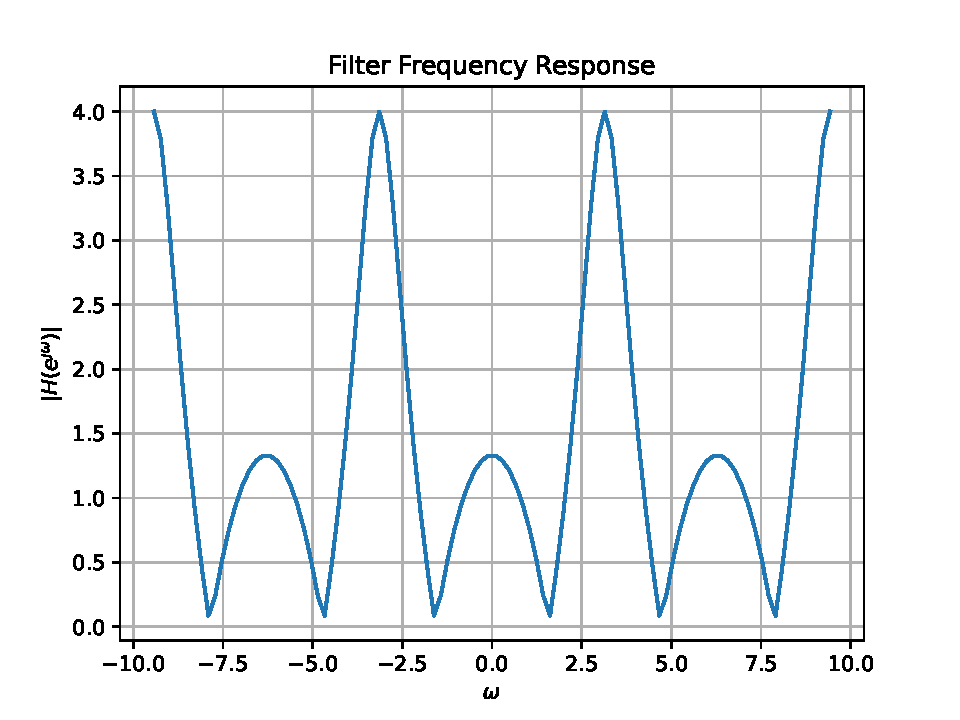
\includegraphics[width=\columnwidth]{figs/4.5 dtft}
\caption{$\abs{H\brak{e^{\j\omega}}}$}
\label{fig:dtft}
\end{figure}
\begin{align}
	\left|H\brak{e^{\j\omega}}\right| &= \left|\frac{1 + e^{-2\j\omega}}{1 + \frac{1}{2}e^{-\j\omega}}\right| \\
									  &= \sqrt{\frac{\brak{1 + \cos{2\omega}}^2 + \brak{\sin{2\omega}}^2}{\brak{1 + \frac{1}{2}\cos{\omega}}^2 + \brak{\frac{1}{2}\sin{\omega}}^2}}\\
					0				  &= \sqrt{\frac{2\brak{1 + \cos{2\omega}}}{\frac{5}{4} + \cos{\omega}}} \\
									  &= \sqrt{\frac{2\brak{2\cos^2{\omega}}}{\frac{5}{4} + \cos{\omega}}} \\
									  &= \frac{4|\cos{\omega}|}{\sqrt{5 + 4\cos{\omega}}}
\end{align}
and so its fundamental period is $2\pi$.
\item Express $x(n)$ in terms of $H\brak{e^{j \omega}}$.\\
\solution
\begin{align}
     h(n) &= \frac{1}{2\pi} \int_{-\pi}^{\pi} H\brak{e^{\j \omega}}e^{j\omega n} \,d\omega \\
     &= \frac{1}{2\pi} \int_{-\pi}^{\pi} \frac{1 + e^{-2\j\omega}}{1 + \frac12 e^{-\j\omega}} e^{j\omega n} \,d\omega 
\end{align}
\end{enumerate}
\section{Impulse Response}
\begin{enumerate}[label=\thesection.\arabic*]
	\item Using long division, 
find
		\begin{align}
			h(n), \quad n < 5
		\end{align}
		for H(z) in 
		\eqref{eq:freq_resp}.
\solution\\
\begin{align}
	H(z) &= \frac{1 + z^{-2}}{1 + \frac{1}{2}z^{-1}} \\
	1+z^{-2} &= \left(1 + \frac{1}{2}z^{-1}\right)*\left(2z^{-1}-4\right) + 5 \\
	H(z)&= \frac{\left(1 + \frac{1}{2}z^{-1}\right)*\left(2z^{-1}-4\right) + 5}{1 + \frac{1}{2}z^{-1}} \\
	&= 2z^{-1}-4 + \frac{5}{1 + \frac{1}{2}z^{-1}}
\end{align}
Now,
\begin{align}
	\frac{5}{1 + \frac{1}{2}z^{-1}} &= 5\left(1-\frac{z^{-1}}{2}+\frac{z^{-2}}{4}-\frac{z^{-3}}{8}+\dots\right) \\
	&= 5-\frac{5}{2}z^{-1}+\frac{5}{4}z^{-2}-\frac{5}{8}z^{-3}+\dots \\
	&= \sum_{n = 0}^{\infty}  5 \left(\frac{-z^{-1}}{2}\right)^n
\end{align}
\begin{align}
	H(z)&= 2z^{-1}-4 + \frac{5}{1 + \frac{1}{2}z^{-1}} \\
	&= 2z^{-1}-4 + \sum_{n = 0}^{\infty}  5 \left(\frac{-z^{-1}}{2}\right)^n 
\end{align}
As $n<5$,
\begin{align}
	H(z) &= 2z^{-1}-4 + \sum_{n = 0}^{4}  5 \left(\frac{-z^{-1}}{2}\right)^n \\
	H(z) &= 1-\frac{1}{2}z^{-1}+\frac{5}{4}z^{-2}-\frac{5}{8}z^{-3}+\frac{5}{16}z^{-4} \\
	\implies h(n) &= \brak{1, \frac{-1}{2}, \frac{5}{4}, \frac{-5}{8}, \frac{5}{16}}
\end{align}
for general n,
\begin{align}
	% h(n) = 2z^{-1}-4+\sum_{n = 0}^{\infty}  5 \left(\frac{-z^{-1}}{2}\right)^{n-2} \\
	h(n) = 
	\begin{cases}
		 1 & n = 0 \\
		 -\dfrac{1}{2} & n = 1 \\
		 \dfrac{3}{2} \brak{-\dfrac12}^{n-2} & n \ge 2
	\end{cases}
\end{align}
		
\item \label{prob:impulse_resp}
Find an expression for $h(n)$ using $H(z)$, given that 
%in Problem \ref{eq:ztransab} and \eqref{eq:anun}, given that
\begin{equation}
\label{eq:impulse_resp}
h(n) \ztrans H(z)
\end{equation}
and there is a one to one relationship between $h(n)$ and $H(z)$. $h(n)$ is known as the {\em impulse response} of the
system defined by \eqref{eq:iir_filter}.
\\
\solution From \eqref{eq:freq_resp},
\begin{align}
H(z) &= \frac{1}{1 + \frac{1}{2}z^{-1}} + \frac{ z^{-2}}{1 + \frac{1}{2}z^{-1}}
\\
\implies h(n) &= \brak{-\frac{1}{2}}^{n}u(n) + \brak{-\frac{1}{2}}^{n-2}u(n-2)
\end{align}
using \eqref{eq:anun} and \eqref{eq:z_trans_shift}.
\item Sketch $h(n)$. Is it bounded? Convergent? 
\\
\solution The following code plots Fig. \ref{fig:hn}.
\begin{lstlisting}
	https://github.com/shreyaswankhede12/EE3900/blob/master/Assignment%201/codes/qs%205/hn.py
\end{lstlisting}
\begin{figure}[!ht]
\centering
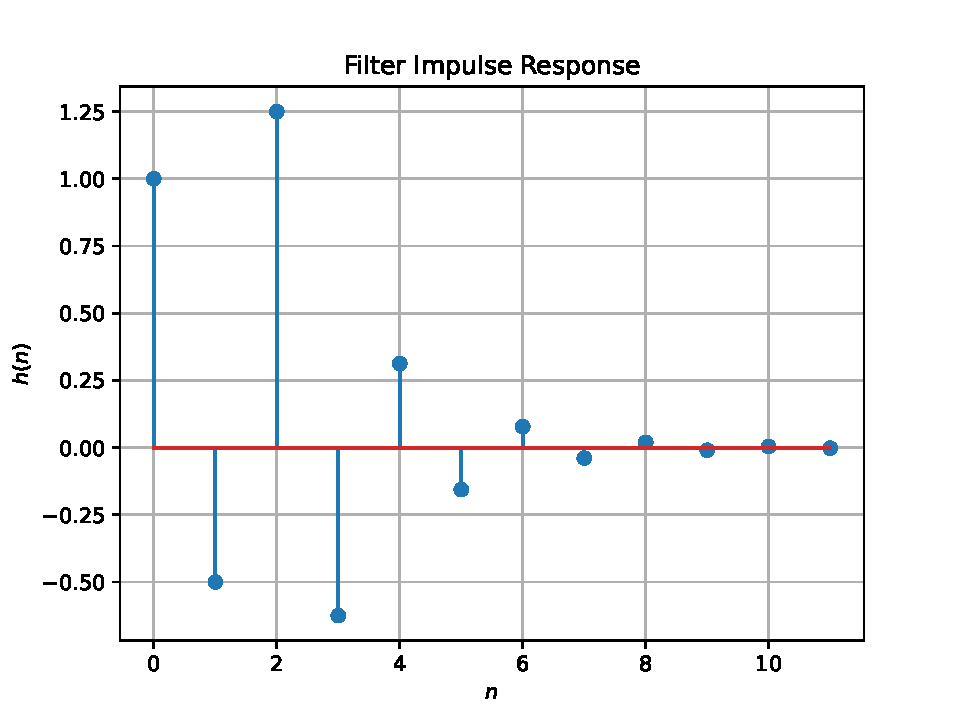
\includegraphics[width=\columnwidth]{figs/5.2 hn}
\caption{$h(n)$ as the inverse of $H(z)$}
\label{fig:hn}
\end{figure}
The sequence is convergnet to $0$ and hence bounded as well.
%
\item Convergent? Justify using the ratio test.\\
\solution Using the ratio test for convergence
	\begin{align}
		\lim_{n \to \infty} \abs{\frac{h(n+1)}{h(n)}} &= \lim_{n \to \infty} \abs{\frac{\brak{-\frac12}^{n-1} \brak{\frac14 + 1}}{\brak{-\frac12}^{n-2} \brak{\frac14 + 1}}} \\
		&= \lim_{n \to \infty} \abs{-\frac12} \\
		&= \frac{1}{2} < 1
	\end{align}
	Therefore, $h(n)$ is convergent.
\item The system with $h(n)$ is defined to be stable if
\begin{equation}
\sum_{n=-\infty}^{\infty}h(n) < \infty
\end{equation}
Is the system defined by \eqref{eq:iir_filter} stable for the impulse response in \eqref{eq:impulse_resp}?\\
%
\solution
	\begin{multline}
		\sum_{n=-\infty}^{\infty}h(n) = \sum_{n=-\infty}^{\infty} \brak{-\frac12}^n u(n) \\
		+ \sum_{n=-\infty}^{\infty} \brak{-\frac12}^{n-2} u(n-2)
	\end{multline}
	\begin{align}
		\sum_{n=-\infty}^{\infty}h(n) = \sum_{n=0}^{\infty}\brak{-\frac12}^n + \sum_{n=2}^{\infty}\brak{-\frac12}^{n-2}
	\end{align}
	
	\begin{align}
		\sum_{n=-\infty}^{\infty}h(n) &= \frac{1}{1 - \brak{-\frac12}} + \frac{1}{1 - \brak{-\frac12}} \\
		&= \frac{4}{3} < \infty
	\end{align}
	
	Therefore, the system is stable.
\item Verify the above result using a python code.
\solution :\\
\begin{lstlisting}
	https://github.com/shreyaswankhede12/EE3900/blob/master/Assignment%201/codes/qs%205/5.6.py
\end{lstlisting}
\item 
Compute and sketch $h(n)$ using 
\begin{equation}
\label{eq:iir_filter_h}
h(n) + \frac{1}{2}h(n-1) = \delta(n) + \delta(n-2), 
\end{equation}
%
This is the definition of $h(n)$.
\\
\solution \begin{equation}
	\label{eq:iir_filter_h}
	h(n) + \frac{1}{2}h(n-1) = \delta(n) + \delta(n-2), 
	\end{equation}
	%
	This is the definition of $h(n)$.
	\\
	\begin{equation}
		 h(0) = 1
	\end{equation}
	Now, for $n = 1$,
	\begin{align}
		 h(1) + \frac12 h(0) &= \delta(1) + \delta(-1) = 0 \\
		 \implies h(1) &= - \frac{1}{2} h(0) = -\frac{1}{2}
	\end{align}
	For $n = 2$,
	\begin{align}
		 h(2) + \frac12 h(1) &= \delta(2) + \delta(0) = 1 \\
		 \implies h(2) &= 1 - \frac{1}{2} h(1) = \frac{5}{4}
	\end{align}
	For $n > 2$, the right hand side of the equation is always zero. Thus,
	\begin{align}
		 h(n) &= -\frac{1}{2} h(n-1) \qquad n > 2 \\
		 h(3) &= \frac{5}{4} \brak{-\frac12} \\
		 h(4) &= \frac{5}{4} \brak{-\frac12}^2 \\
		 &~\vdots \\
		 h(n) &= \frac{5}{4} \brak{-\frac12}^{n-2}
	\end{align}
	Therefore,
	\begin{align}
		 h(n) = 
		 \begin{cases}
			  1 & n = 0 \\
			  -\dfrac{1}{2} & n = 1 \\
			  \dfrac{5}{4} \brak{-\dfrac12}^{n-2} & n \ge 2
		 \end{cases}
	\end{align}
	Thus, it is bounded and convergent to $0$
	\begin{equation}
		 \lim_{n \to \infty} h(n) = 0
	\end{equation} 
The following code plots Fig. \ref{fig:hndef}. Note that this is the same as Fig. 
\ref{fig:hn}. 
%
\begin{lstlisting}
	https://github.com/shreyaswankhede12/EE3900/blob/master/Assignment%201/codes/qs%205/hndef.py
\end{lstlisting}
\begin{figure}[!ht]
\centering
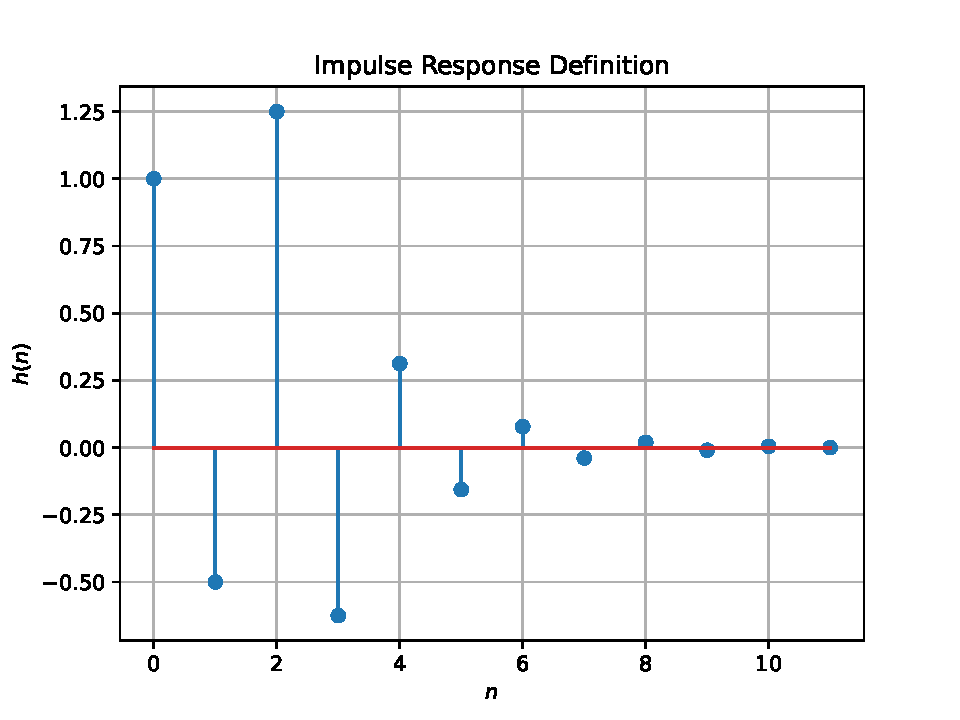
\includegraphics[width=\columnwidth]{figs/5.4 hndef}
\caption{$h(n)$ from the definition}
\label{fig:hndef}
\end{figure}
%
\item Compute 
%
\begin{equation}
\label{eq:convolution}
y(n) = x(n)*h(n) = \sum_{n=-\infty}^{\infty}x(k)h(n-k)
\end{equation}
%
Comment. The operation in \eqref{eq:convolution} is known as
{\em convolution}.\\
\solution
	\begin{align}
		x(n)*h(n) &= \sum_{k=-\infty}^{\infty}x(k)h(n-k) \\
		&= \sum_{k=0}^{5}x(k)h(n-k)
	\end{align}
%
\\
\solution The following code plots Fig. \ref{fig:ynconv}. Note that this is the same as 
$y(n)$ in  Fig. 
\ref{fig:xnyn}. 
%
\begin{lstlisting}
	https://github.com/shreyaswankhede12/EE3900/blob/master/Assignment%201/codes/qs%205/ynconv.py
\end{lstlisting}
\begin{figure}[!ht]
\centering
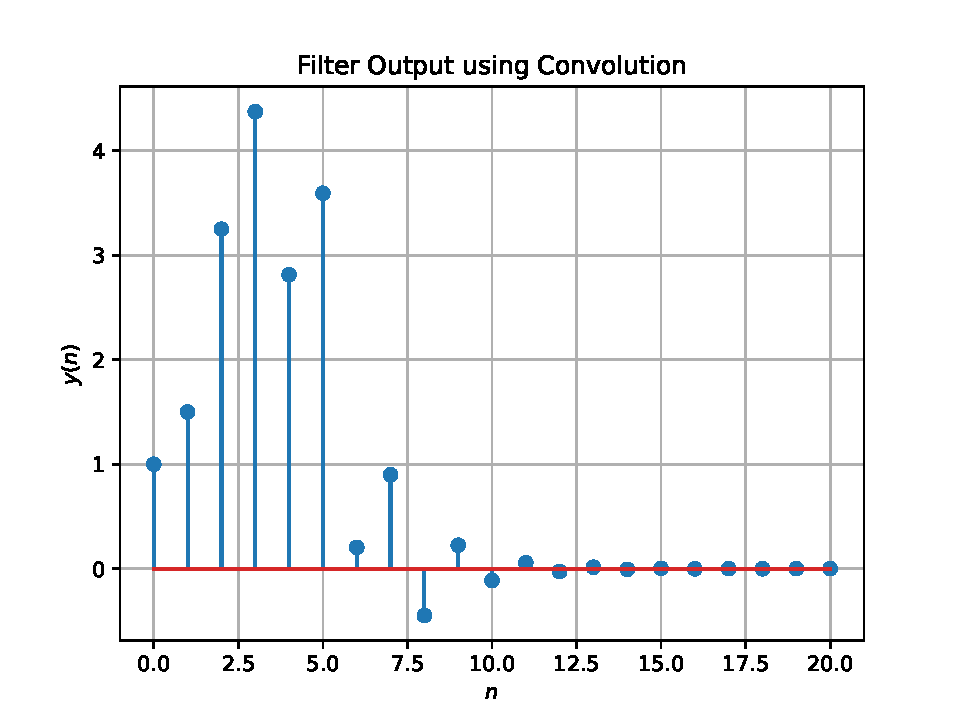
\includegraphics[width=\columnwidth]{figs/5.5 ynconv}
\caption{$y(n)$ from the definition of convolution}
\label{fig:ynconv}
\end{figure}
\item Express the above convolution using a Teoplitz matrix.\\
\solution
\begin{align}
    \vec{x} &= \myvec{1 & 2	 & 3 & 4 & 2 & 1}^\top \\
	\vec{h} &= \myvec{h_0 & h_1	 & \cdots & h_{N-1}}^\top \\
     \vec{y} &= \vec{x} \circledast \vec{h} \\
	\myvec{y_1 \\ y_2 \\ \vdots \\ y_{N+5}} &= \myvec{
			h_0 & 0 & 0 & \cdots & 0 \\
			h_1 & h_0 & 0 & \cdots & 0 \\
			h_2 & h_1 & h_0 & \cdots & 0 \\
			\vdots & \vdots & \vdots & \ddots & \vdots \\
			h_{N-1} & h_{N-2} & h_{N-3} & \cdots & h_{N-6} \\
			0 & h_{N-1} & h_{N-2} & \cdots & h_{N-5} \\
			0 & 0 & h_{N-1} & \cdots & h_{N-4} \\
			\vdots & \vdots & \vdots & \ddots & \vdots \\
			0 & 0 & 0 & \cdots & h_{N-1} }
               \myvec{1.0\\2.0\\3.0\\4.0\\2.0\\1.0}
\end{align}
\item Show that
\begin{equation}
y(n) =  \sum_{n=-\infty}^{\infty}x(n-k)h(k)
\end{equation}
\solution We know that
	\begin{equation}
		y(n) = x(n)*h(n) = \sum_{k=-\infty}^{\infty}x(k)h(n-k)
	\end{equation}
	
	Substitute $k = n - i$
	\begin{align}
		 \sum_{k=-\infty}^{\infty}x(k)h(n-k) &=  \sum_{n - i =-\infty}^{\infty}x(n-i)h(n-(n-i)) \\
		 &= \sum_{i = \infty}^{-\infty} x(n - i) h(i) \\
		 &= \sum_{i = -\infty}^{\infty} x(n - i) h(i)
	\end{align}
	since the order of limits does not matter for a summation.
	Thus,
	\begin{align}
		\sum_{k=-\infty}^{\infty}x(k)h(n-k) &= \sum_{k=-\infty}^{\infty}x(n-k)h(k) \\
		\implies x(n) * h(n) &= h(n) * x(n)
	\end{align}

\end{enumerate}
%
\section{DFT and FFT}
\begin{enumerate}[label=\thesection.\arabic*]
\item
Compute
\begin{equation}
X(k) \define \sum _{n=0}^{N-1}x(n) e^{-\j2\pi kn/N}, \quad k = 0,1,\dots, N-1
\end{equation}
and $H(k)$ using $h(n)$.\\
\solution Download the following Python code that plots Fig. \ref{fig-6.1}.
\begin{lstlisting}
		https://github.com/shreyaswankhede12/EE3900/blob/master/Assignment%201/codes/qs%206/6.1.py		
\end{lstlisting}
	
	Run the code by executing
	\begin{lstlisting}
		python 6.1.py
	\end{lstlisting}

	\begin{figure}[!ht]
		\centering
		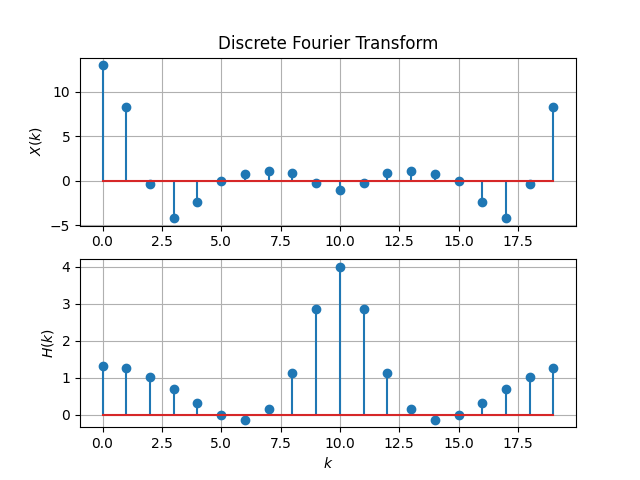
\includegraphics[width=\columnwidth]{figs/6.1.png}
		\caption{Plots of the real parts of the discrete Fourier transforms of $x(n)$ and $h(n)$}
		\label{fig-6.1}	
	\end{figure}
\item Compute 
\begin{equation}
Y(k) = X(k)H(k)
\end{equation}
\solution Download the following Python code that plots Fig. \ref{fig-6.2}.
	\begin{lstlisting}
		https://github.com/shreyaswankhede12/EE3900/blob/master/Assignment%201/codes/qs%206/6.2.py
	\end{lstlisting}
	
	Run the code by executing
	\begin{lstlisting}
		python 6.2.py
	\end{lstlisting}

	\begin{figure}[!ht]
		\centering
		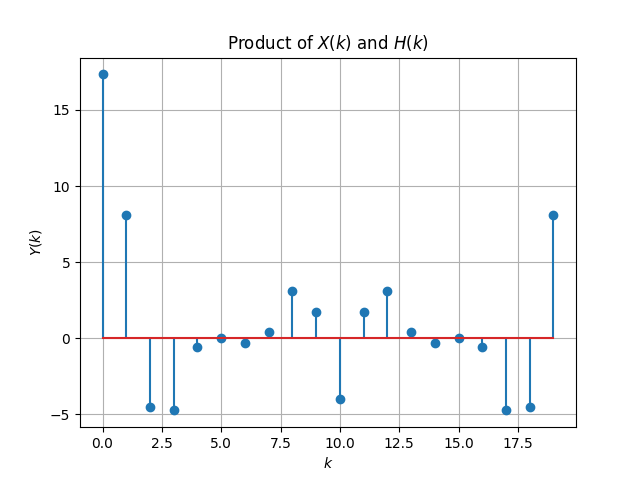
\includegraphics[width=\columnwidth]{figs/6.2.png}
		\caption{Plot of $Y(k)$}
		\label{fig-6.2}	
	\end{figure}

\item Compute
\begin{equation}
 y\brak{n}={\frac {1}{N}}\sum _{k=0}^{N-1}Y\brak{k}\cdot e^{\j 2\pi kn/N},\quad n = 0,1,\dots, N-1
\end{equation}
\\
\solution Download the following Python code that plots Fig. \ref{fig-6.3}.
	\begin{lstlisting}
		https://github.com/shreyaswankhede12/EE3900/blob/master/Assignment%201/codes/qs%206/6.3.py
	\end{lstlisting}
	
	Run the code by executing
	\begin{lstlisting}
		python 6.3.py
	\end{lstlisting}

	\begin{figure}[!ht]
		\centering
		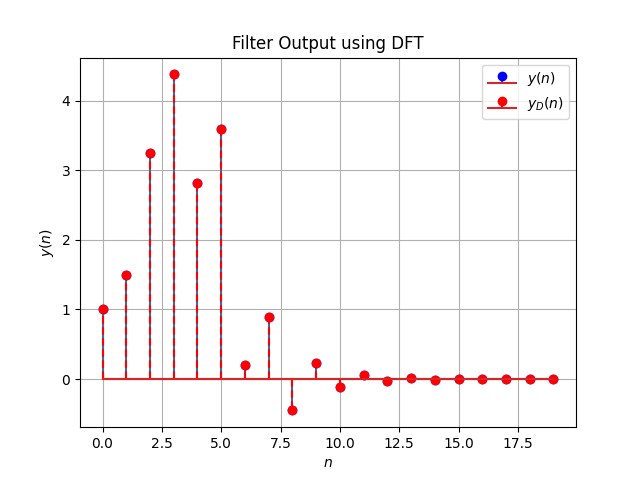
\includegraphics[width=\columnwidth]{figs/6.3.png}
		\caption{Plot of the inverse discrete Fourier transform of $Y(k)$}
		\label{fig-6.3}	
	\end{figure}
	
	The plot is exactly the same as that obtained in Fig. 3.2. Therefore, we conclude that 
	\begin{align}
		y(n) &= x(n) * h(n) \\
		\iff Y(k) &= X(k)H(k)
	\end{align}
\item Repeat the previous exercise by computing $X(k), H(k)$ and $y(n)$ through FFT and 
IFFT.\\
\solution Download the following Python code that plots Fig. \ref{fig-6.4}.
	\begin{lstlisting}
		https://github.com/shreyaswankhede12/EE3900/blob/master/Assignment%201/codes/qs%206/6.4.py
	\end{lstlisting}
	
	Run the code by executing
	\begin{lstlisting}
		python 6.4.py
	\end{lstlisting}

	\begin{figure}[!ht]
		\centering
		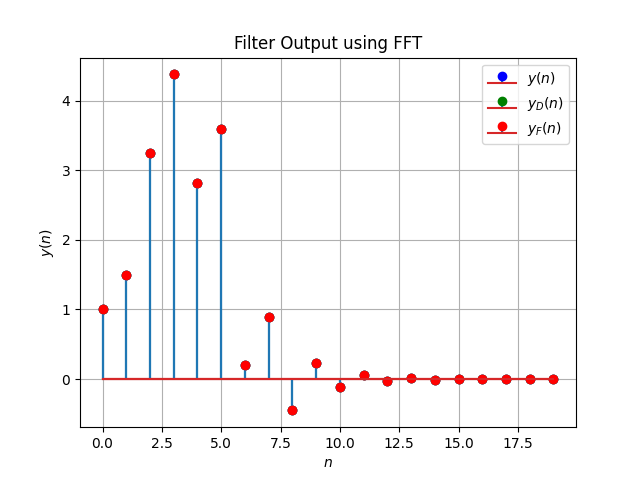
\includegraphics[width=\columnwidth]{./figs/6.4.png}
		\caption{Plot of $y(n)$ by fast Fourier transform}
		\label{fig-6.4}	
	\end{figure}
	
	The plot is exactly the same as that obtained in Fig. 3.2.
\item Wherever possible, express all the above equations as matrix equations.\\
\solution
	\begin{align}
		\vec{x} &= \myvec{x_0 & x_1	 & \cdots & x_{N-1}}^\top \\
		\vec{h} &= \myvec{x_0 & x_1	 & \cdots & x_{N-1}}^\top \\
		\vec{y} &= \vec{x} \circledast \vec{h} \\
		\myvec{y_1 \\ y_2 \\ \vdots \\ y_{2N - 1}} &= \myvec{
			h_0 & 0 & 0 & \cdots & 0 \\
			h_1 & h_0 & 0 & \cdots & 0 \\
			h_2 & h_1 & h_0 & \cdots & 0 \\
			\vdots & \vdots & \vdots & \ddots & \vdots \\
			h_{N-1} & h_{N-2} & h_{N-3} & \cdots & h_0 \\
			0 & h_{N-1} & h_{N-2} & \cdots & h_1 \\
			0 & 0 & h_{N-1} & \cdots & h_2 \\
			\vdots & \vdots & \vdots & \ddots & \vdots \\
			0 & 0 & 0 & \cdots & h_{N-1}
		}		
		\myvec{x_1\\x_2\\ \vdots \\x_N}
	\end{align}
	
	The convolution can be written using a Toeplitz matrix. 
	
	Consider the DFT matrix
	\begin{align}
		\vec{W} = \myvec{
			1 & 1 & 1 & 1 & \cdots & 1 \\
			1 & \omega & \omega^2 & \omega^3 & \cdots & \omega^{N-1} \\
			1 & \omega^2 & \omega^4 & \omega^6 & \cdots & \omega^{2(N-1)} \\
			1 & \omega^3 & \omega^6 & \omega^9 & \cdots & \omega^{3(N-1)} \\
			\vdots & \vdots & \vdots & \vdots & \ddots & \vdots \\ 
			1 & \omega^{N-1} & \omega^{2(N-1)} & \omega^{3(N-1)} & \cdots & \omega^{(N-1)(N-1)}
		}
	\end{align}
	
	where $\omega = e^{-\j 2\pi/N}$ is the $N^{\mathrm{th}}$ root of unity
	
	Then the discrete Fourier transforms of $\vec{x}$ and $\vec{h}$ are given by
	\begin{align}
		\vec{X} &= \vec{W} \vec{x} \\
		\vec{H} &= \vec{W} \vec{h}
	\end{align}
	
	$\vec{Y}$ is then given by
	\begin{equation}
		\vec{Y} = \vec{X} \circ \vec{H}
	\end{equation}
	where $\circ$ denotes the Hadamard product (element-wise multiplication)
	
	But $\vec{Y}$ is the discrete Fourier transform of the filter output $\vec{y}$
	\begin{equation}
		\vec{Y} = \vec{W} \vec{y}
	\end{equation}
	
	Thus,
	\begin{align}
		\vec{W} \vec{y} &= \vec{X} \circ \vec{H} \\
		\implies \vec{y} &= \vec{W}^{-1} \brak{\vec{X} \circ \vec{H}} \\
		&= \vec{W}^{-1} \brak{\vec{W} \vec{x} \circ \vec{W} \vec{h}}
	\end{align}
\end{enumerate}
%
\section{FFT}
% \subsection{Definitions}
\begin{enumerate}[label=\arabic*.,ref=\thesection.\theenumi]
\numberwithin{equation}{section}
    \item The DFT of $x(n)$ is given by
    \begin{align}
        X(k) \triangleq \sum_{n=0}^{N-1} x(n) e^{-j 2 \pi k n / N}, \quad k=0,1, \ldots, N-1
    \end{align}
\item Let 
	\begin{align}
W_{N} = e^{-j2\pi/N} 
	\end{align}
		Then the $N$-point {\em DFT matrix} is defined as 
	\begin{align}
		\vec{F}_{N} = \sbrak{W_{N}^{mn}}, \quad 0 \le m,n \le N-1 
	\end{align}
	where $W_{N}^{mn}$ are the elements of $\vec{F}_{N}$.
\item Let 
	\begin{align}
		\vec{I}_4 = \myvec{\vec{e}_4^{1} &\vec{e}_4^{2} &\vec{e}_4^{3} &\vec{e}_4^{4} }
	\end{align}
		be the $4\times 4$ identity matrix.  Then the 4 point {\em DFT permutation matrix} is defined as 
	\begin{align}
		\vec{P}_4 = \myvec{\vec{e}_4^{1} &\vec{e}_4^{3} &\vec{e}_4^{2} &\vec{e}_4^{4} }
	\end{align}
\item The 4 point {\em DFT diagonal matrix} is defined as 
	\begin{align}
		\vec{D}_4 = diag\myvec{W_{8}^{0} & W_{8}^{1} & W_{8}^{2} & W_{8}^{3}}
	\end{align}
\item Show that 
\begin{equation}
    W_{N}^{2}=W_{N/2}
\end{equation}
\solution
	\begin{align}
		W_N^2 &= \brak{\exp\brak{-j\frac{2\pi}{N}}}^2	 \\
		&= \exp\brak{-j\frac{2\pi}{N} \cdot 2} \\
		&= \exp\brak{-j\frac{2\pi}{N/2}} \\
		&= W_{N/2}
	\end{align}	 
%    \item Find $\vec{P}_6$.
%    \item Find $\vec{D}_3$.
    \item Show that 
\begin{equation}
	\vec{F}_{4}=
\begin{bmatrix}
	\vec{I}_{2} & \vec{D}_{2} \\
\vec{I}_{2} & -\vec{D}_{2}
\end{bmatrix}
\begin{bmatrix}
\vec{F}_{2} & 0 \\
0 & \vec{F}_{2}
\end{bmatrix}
\vec{P}_{4}
\end{equation}
\solution
	\begin{align}
		&\mymat{\vec{I}_2 & \vec{D}_2 \\ \vec{I}_2 & -\vec{D}_2} \mymat{\vec{F}_2 & 0 \\ 0 & \vec{F}_2} \\
		= &\mymat{\vec{F}_2 & \vec{D}_2\vec{F}_2 \\ \vec{F}_2 & -\vec{D}_2\vec{F}_2}  \\
		= &\mymat{\myvec{1&1\\1&-1} & \myvec{1&0\\0&-\j}\myvec{1&1\\1&-1} \\ \myvec{1&1\\1&-1} & - \myvec{1&0\\0&-\j}\myvec{1&1\\1&-1}} \\
		= &\mymat{1 & 1 & 1 & 1 \\ 1 & -1 & -\j & \j \\ 1 & 1 & -1 & -1 \\ 1 & -1 & \j & -\j}
	\end{align}		
	because $W_2^0 = 1$ and $W_2^1 = e^{-\j\pi} = -1$
	
	Now
	\begin{align}
		&\mymat{\vec{I}_2 & \vec{D}_2 \\ \vec{I}_2 & -\vec{D}_2} \mymat{\vec{F}_2 & 0 \\ 0 & \vec{F}_2} \vec{P}_4 \\
		= &\mymat{1 & 1 & 1 & 1 \\ 1 & -1 & -\j & \j \\ 1 & 1 & -1 & -1 \\ 1 & -1 & \j & -\j} \mymat{1 & 0 & 0 & 0 \\ 0 & 0 & 1 & 0 \\ 0 & 1 & 0 & 0 \\ 0 & 0 & 0 & 1} \\
		= &\mymat{1 & 1 & 1 & 1 \\ 1 & -\j & -1 & \j \\ 1 & -1 & 1 & -1 \\ 1 & \j & -1 & -\j} \\
		= &\mymat{W_4^0 & W_4^0 & W_4^0 & W_4^0 \\ W_4^0 & W_4^1 & W_4^2 & W_4^3 \\ W_4^0 & W_4^2 & W_4^4 & W_4^6 \\ W_4^0 & W_4^3 & W_4^6 & W_4^9} \\
		= &~\vec{F}_4
	\end{align}
	because
	\begin{align}
		W_4^0 &= 1 \\
		W_4^1 &= e^{-\j\frac{\pi}{2}} = -\j \\
		W_4^2 &= e^{-\j\pi} = -1 \\
		W_4^3 &= e^{-\j\frac{3\pi}{2}} = \j \\
		W_4^n &= W_4^{n - 4} &&\forall n \ge 4
	\end{align}	
	\item Show that 
\begin{equation}
\vec{F}_{N}=
\begin{bmatrix}
\vec{I}_{N/2} & \vec{D}_{N/2} \\
\vec{I}_{N/2} & -\vec{D}_{N/2}
\end{bmatrix}
\begin{bmatrix}
\vec{F}_{N/2} & 0 \\
0 & \vec{F}_{N/2}
\end{bmatrix}
\vec{P}_{N}
\end{equation}

	\solution
	\begin{align}
		&\mymat{\vec{I}_{N/2} & \vec{D}_{N/2} \\ \vec{I}_{N/2} & -\vec{D}_{N/2}} \mymat{\vec{F}_{N/2} & 0 \\ 0 & \vec{F}_{N/2}}  \\
		= &\mymat{\vec{F}_{N/2} & \vec{D}_{N/2}\vec{F}_{N/2} \\ \vec{F}_{N/2} & -\vec{D}_{N/2}\vec{F}_{N/2}}
	\end{align}
	
	Now
	\begin{align}
		&\vec{D}_{N/2}\vec{F}_{N/2} \\
		&= \mymat{W_N^0 & \cdots & 0 \\ \vdots & \ddots & \vdots \\ 0 & \cdots & W_N^{N/2-1}} \mymat{W_{N/2}^0 & \cdots & W_{N/2}^0 \\ \vdots & \ddots & \vdots \\ W_{N/2}^0 & \cdots & W_{N/2}^{(N/2 - 1)^2}} \\
		&= \mymat{W_N^0 W_{N/2}^0 & \cdots & W_N^0 W_{N/2}^0 \\ \vdots & \ddots & \vdots \\ W_N^{N/2-1} W_{N/2}^0 & \cdots & W_N^{N/2-1} W_{N/2}^{(N/2 - 1)^2}} 
	\end{align}
	
	Thus
	\begin{align}
		\brak{\vec{D}_{N/2}\vec{F}_{N/2}}_{ij} &= W_N^i W_{N/2}^{ij} \\
		&= W_N^i W_N^{2ij} \\
		&= W_N^{i(2j + 1)}
	\end{align}
	where $i, j = 0, \ldots, N/2 - 1$
	
	Therefore, $\vec{D}_{N/2}\vec{F}_{N/2}$ forms the first $N/2$ rows of the odd-indexed columns of $\vec{F}_N$
	\begin{align}
		W_N^{(i + N/2)(2j + 1)} &= \exp\brak{-\j \frac{2\pi}{N} (2j + 1)\brak{i + \frac{N}{2}}} \\
		&= \exp\brak{-\j \brak{\frac{2\pi}{N} (2j + 1)i + (2j + 1)\pi}} \\
		&= -\exp\brak{-\j \frac{2\pi}{N} (2j + 1)i} \\
		&= -W_N^{i(2j + 1)}
	\end{align}
	
	Thus, the remaining $N/2$ rows will be the negatives of the first $N/2$ rows
	\begin{align}
		\brak{\vec{F}_{N/2}}_{ij} &= W_{N/2}^{ij} \\
		&= W_N^{i(2j)}
	\end{align}
	where $i, j = 0, \ldots, N/2 - 1$
	
	Therefore, $\vec{F}_{N/2}$ forms the first $N/2$ rows of the even-indexed columns of $\vec{F}_N$
	\begin{align}
		W_N^{(i + N/2)(2j)} &= \exp\brak{-\j \frac{2\pi}{N} (2j)\brak{i + \frac{N}{2}}} \\
		&= \exp\brak{-\j \brak{\frac{2\pi}{N} (2j)i + (2j)\pi}} \\
		&= \exp\brak{-\j \frac{2\pi}{N} (2j)i} \\
		&= W_N^{i(2j)}
	\end{align}
	Thus, the remaining $N/2$ rows will be the same as the first $N/2$ rows
	
	Therefore
	\begin{align}
		\mymat{\vec{F}_{N/2} & \vec{D}_{N/2}\vec{F}_{N/2} \\ \vec{F}_{N/2} & -\vec{D}_{N/2}\vec{F}_{N/2}} = \vec{F}_N \vec{P}_N
	\end{align}
	where 
	\begin{align}
		\vec{P}_N = \myvec{\vec{e}_N^1 & \vec{e}_N^3 & \cdots & \vec{e}_N^{N-1} & \vec{e}_N^2 & \vec{e}_N^4 & \cdots & \vec{e}_N^N}
	\end{align}
	
	Hence
	\begin{align}
		\mymat{\vec{F}_{N/2} & \vec{D}_{N/2}\vec{F}_{N/2} \\ \vec{F}_{N/2} & -\vec{D}_{N/2}\vec{F}_{N/2}} \vec{P}_N = \vec{F}_N \vec{P}_N^2 = \vec{F}_N \\
		\therefore \vec{F}_N = \mymat{\vec{I}_{N/2} & \vec{D}_{N/2} \\ \vec{I}_{N/2} & -\vec{D}_{N/2}} \mymat{\vec{F}_{N/2} & 0 \\ 0 & \vec{F}_{N/2}} \vec{P}_N
	\end{align}
	for even $N$
	\item Find 
    \begin{align}
	     \vec{P}_4 \vec{x}
    \end{align}
    
    \solution Let $\vec{x} = \myvec{x(0) & x(1) & x(2) & x(3)}^\top$
    \begin{align}
		\vec{P}_4 \vec{x} &= \mymat{1 & 0 & 0 & 0 \\ 0 & 0 & 1 & 0 \\ 0 & 1 & 0 & 0 \\ 0 & 0 & 0 & 1} \mymat{x(0) \\ x(1) \\ x(2) \\ x(3)} \\
		&= \mymat{x(0) \\ x(2) \\ x(1) \\ x(3)}
    \end{align}

\item Show that 
    \begin{align}
	    \vec{X} = \vec{F}_N \vec{x}
	    \label{eq:dft-mat-def}
    \end{align}
		where $\vec{x}, \vec{X}$ are the vector representations of $x(n), X(k)$ respectively.
		
	\solution
	\begin{align}
        X(k) &= \sum_{n=0}^{N-1} x(n) e^{-j 2 \pi k n / N}, \quad k=0,1, \ldots, N-1 \\
        \implies \vec{X} &= \mymat{\sum_{n=0}^{N-1} x(n) e^{-j 2 \pi  n (0) / N} \\ \vdots \\ \sum_{n=0}^{N-1} x(n) e^{-j 2 \pi  n (N-1) / N}} \\
        &= \mymat{x(0) + \cdots + x(N-1) \\ \vdots \\ x(0) + \cdots + x(N-1) e^{-j 2 \pi (N-1)^2 / N}} 
    \end{align}
    \begin{align}
    		\vec{X} &= x(0) \mymat{1 \\ \vdots \\ 1} + \cdots + x(N-1)\mymat{1 \\ \vdots \\ e^{-j 2 \pi (N-1)^2 / N}} \\
    		&= \mymat{1 & \cdots & 1 \\ \vdots & \ddots & \vdots \\ 1 & \cdots & e^{-j 2 \pi (N-1)^2 / N}} \mymat{x(0) \\ \vdots \\ x(N-1)} \\
    		&= \vec{F}_N \vec{x}
    \end{align}
		
\item Derive the following step-by-step visualisation  of
8-point FFTs into 4-point FFTs and so on
\begin{equation}
\begin{bmatrix}
X(0) \\ 
X(1) \\ 
X(2) \\ 
X(3)
\end{bmatrix}
=
\begin{bmatrix}
X_{1}(0) \\ 
X_{1}(1)\\ 
X_{1}(2)\\
X_{1}(3)\\
\end{bmatrix}
+
\begin{bmatrix}
W^{0}_{8} & 0 & 0 & 0\\
0 & W^{1}_{8} & 0 & 0\\
0 & 0 & W^{2}_{8} & 0\\
0 & 0 & 0 & W^{3}_{8}
\end{bmatrix}
\begin{bmatrix}
X_{2}(0) \\ 
X_{2}(1) \\ 
X_{2}(2) \\
X_{2}(3)
\end{bmatrix}
\end{equation}
\begin{equation}
\begin{bmatrix}
X(4) \\ 
X(5) \\ 
X(6) \\ 
X(7)
\end{bmatrix}
=
\begin{bmatrix}
X_{1}(0) \\ 
X_{1}(1)\\ 
X_{1}(2)\\
X_{1}(3)\\
\end{bmatrix}
-
\begin{bmatrix}
W^{0}_{8} & 0 & 0 & 0\\
0 & W^{1}_{8} & 0 & 0\\
0 & 0 & W^{2}_{8} & 0\\
0 & 0 & 0 & W^{3}_{8}
\end{bmatrix}
\begin{bmatrix}
X_{2}(0) \\ 
X_{2}(1) \\ 
X_{2}(2) \\
X_{2}(3)
\end{bmatrix}
\end{equation}
4-point FFTs into 2-point FFTs
\begin{equation}
\begin{bmatrix}
X_{1}(0) \\ 
X_{1}(1)\\ 
\end{bmatrix}
=
\begin{bmatrix}
X_{3}(0) \\ 
X_{3}(1)\\ 
\end{bmatrix}
+
\begin{bmatrix}
W^{0}_{4} & 0\\
0 & W^{1}_{4}
\end{bmatrix}
\begin{bmatrix}
X_{4}(0) \\ 
X_{4}(1) \\ 
\end{bmatrix}
\end{equation}
\begin{equation}
\begin{bmatrix}
X_{1}(2) \\ 
X_{1}(3)\\ 
\end{bmatrix}
=
\begin{bmatrix}
X_{3}(0) \\ 
X_{3}(1)\\ 
\end{bmatrix}
-
\begin{bmatrix}
W^{0}_{4} & 0\\
0 & W^{1}_{4}
\end{bmatrix}
\begin{bmatrix}
X_{4}(0) \\ 
X_{4}(1) \\ 
\end{bmatrix}
\end{equation}
\begin{equation}
\begin{bmatrix}
X_{2}(0) \\ 
X_{2}(1)\\ 
\end{bmatrix}
=
\begin{bmatrix}
X_{5}(0) \\ 
X_{5}(1)\\ 
\end{bmatrix}
+
\begin{bmatrix}
W^{0}_{4} & 0\\
0 & W^{1}_{4}
\end{bmatrix}
\begin{bmatrix}
X_{6}(0) \\ 
X_{6}(1) \\ 
\end{bmatrix}
\end{equation}
\begin{equation}
\begin{bmatrix}
X_{2}(2) \\ 
X_{2}(3)\\ 
\end{bmatrix}
=
\begin{bmatrix}
X_{5}(0) \\ 
X_{5}(1)\\ 
\end{bmatrix}
-
\begin{bmatrix}
W^{0}_{4} & 0\\
0 & W^{1}_{4}
\end{bmatrix}
\begin{bmatrix}
X_{6}(0) \\ 
X_{6}(1) \\ 
\end{bmatrix}
\end{equation}
\begin{equation}
\vec{P}_{8}
\begin{bmatrix}
x(0) \\ 
x(1) \\ 
x(2) \\ 
x(3) \\ 
x(4) \\ 
x(5) \\
x(6) \\
x(7)
\end{bmatrix}
 = 
\begin{bmatrix}
x(0) \\ 
x(2) \\ 
x(4) \\ 
x(6) \\
x(1) \\ 
x(3) \\ 
x(5) \\
x(7)
\end{bmatrix}
\end{equation}
\begin{equation}
\vec{P}_{4}
\begin{bmatrix}
x(0) \\ 
x(2) \\ 
x(4) \\ 
x(6) \\
\end{bmatrix}
 = 
\begin{bmatrix}
x(0) \\ 
x(4) \\ 
x(2) \\
x(6)
\end{bmatrix}
\end{equation}
\begin{equation}
\vec{P}_{4}
\begin{bmatrix}
x(1) \\ 
x(3) \\ 
x(5) \\
x(7)
\end{bmatrix}
 = 
\begin{bmatrix}
x(1) \\ 
x(5) \\ 
x(3) \\ 
x(7) \\
\end{bmatrix}
\end{equation}
Therefore,
\begin{equation}
\begin{bmatrix}
X_{3}(0) \\ 
X_{3}(1)\\ 
\end{bmatrix}
= \vec{F}_{2}
\begin{bmatrix}
x(0) \\ 
x(4) \\ 
\end{bmatrix}
\end{equation}
\begin{equation}
\begin{bmatrix}
X_{4}(0) \\ 
X_{4}(1)\\ 
\end{bmatrix}
= \vec{F}_{2}
\begin{bmatrix}
x(2) \\ 
x(6) \\ 
\end{bmatrix}
\end{equation}
\begin{equation}
\begin{bmatrix}
X_{5}(0) \\ 
X_{5}(1)\\ 
\end{bmatrix}
= \vec{F}_{2}
\begin{bmatrix}
x(1) \\ 
x(5) \\ 
\end{bmatrix}
\end{equation}
\begin{equation}
\begin{bmatrix}
X_{6}(0) \\ 
X_{6}(1)\\ 
\end{bmatrix}
= \vec{F}_{2}
\begin{bmatrix}
x(3) \\ 
x(7) \\ 
\end{bmatrix}
\end{equation}

	\solution 
	\begin{align}
        X(k) &= \sum_{n=0}^7 x(n) e^{-j 2 \pi k n / 8}, \quad k=0, \ldots, 7\\
        &= \sum_{n=0}^7 x(n) W_8^{kn} \\
        &= \sum_{n \text{ is even}}x(n) W_8^{kn} + \sum_{n \text{ is odd}}x(n) W_8^{kn} \\
        &= \sum_{m=0}^3 x(2m) W_8^{2km} + \sum_{m=0}^3 x(2m+1) W_8^{2km + k}
    \end{align}	
    
    Now substitute $W_8^2 = W_4$
    \begin{align}
    		X(k) = \sum_{m=0}^3 x(2m) W_4^{km} + W_8^k \sum_{m=0}^3 x(2m+1) W_4^{km}
    \end{align}
    
    Consider
    \begin{align}
    		x_1(n) = \cbrak{x(0), x(2), x(4), x(6)} \\
    		x_2(n) = \cbrak{x(1), x(3), x(5), x(7)}
    \end{align}
    
    Thus
    \begin{align}
    		X(k) = X_1(k) + W_8^k X_2(k) \qquad k = 0,\ldots,7
    \end{align}
    
    Now, $X_1(k)$ and $X_2(k)$ are $4$-point DFTs which means they are periodic with period $4$
    \begin{align}
    		X(k+4) &= X_1(k+4) + W_8^{k+4} X_2(k+4) \\
    		&= X_1(k) + e^{-\j 2\pi(k+4)/8} X_2(k) \\
    		&= X_1(k) + e^{-\j (2\pi k/8 + \pi)} X_2(k) \\
    		&= X_1(k) - e^{-\j 2\pi k/8 } X_2(k) \\
    		&= X_1(k) - W_8^k X_2(k)
    \end{align}
    
    Therefore, for $k=0,1,2,3$
    \begin{align}
    		X(k) = X_1(k) + W_8^k X_2(k)  \\
    		X(k+4) = X_1(k) - W_8^k X_2(k) 
    \end{align}
    
    which is the same as
    \begin{equation}
\begin{bmatrix}
X(0) \\ 
X(1) \\ 
X(2) \\ 
X(3)
\end{bmatrix}
=
\begin{bmatrix}
X_{1}(0) \\ 
X_{1}(1)\\ 
X_{1}(2)\\
X_{1}(3)\\
\end{bmatrix}
+
\begin{bmatrix}
W^{0}_{8} & 0 & 0 & 0\\
0 & W^{1}_{8} & 0 & 0\\
0 & 0 & W^{2}_{8} & 0\\
0 & 0 & 0 & W^{3}_{8}
\end{bmatrix}
\begin{bmatrix}
X_{2}(0) \\ 
X_{2}(1) \\ 
X_{2}(2) \\
X_{2}(3)
\end{bmatrix}
\end{equation}
\begin{equation}
\begin{bmatrix}
X(4) \\ 
X(5) \\ 
X(6) \\ 
X(7)
\end{bmatrix}
=
\begin{bmatrix}
X_{1}(0) \\ 
X_{1}(1)\\ 
X_{1}(2)\\
X_{1}(3)\\
\end{bmatrix}
-
\begin{bmatrix}
W^{0}_{8} & 0 & 0 & 0\\
0 & W^{1}_{8} & 0 & 0\\
0 & 0 & W^{2}_{8} & 0\\
0 & 0 & 0 & W^{3}_{8}
\end{bmatrix}
\begin{bmatrix}
X_{2}(0) \\ 
X_{2}(1) \\ 
X_{2}(2) \\
X_{2}(3)
\end{bmatrix}
\end{equation}

	Similarly, we can divide $x_1(n)$ into 
	\begin{align}
		x_3(n) = \cbrak{x(0), x(4)} \\
		x_4(n) = \cbrak{x(2), x(6)}
	\end{align}
	i.e.,
	\begin{align}
		\mymat{X_3(0) \\ X_3(1)} = \vec{F}_2 \mymat{x(0) \\ x(4)} \\
		\mymat{X_4(0) \\ X_4(1)} = \vec{F}_2 \mymat{x(2) \\ x(6)}
	\end{align}
	to get
	\begin{align}
		X_1(k) = X_3(k) + W_4^k X_4(k) \\
		X_1(k + 2) = X_3(k) - W_4^k X_4(k) 
	\end{align}
	for $k = 0, 1$
	\begin{equation}
\begin{bmatrix}
X_{1}(0) \\ 
X_{1}(1)\\ 
\end{bmatrix}
=
\begin{bmatrix}
X_{3}(0) \\ 
X_{3}(1)\\ 
\end{bmatrix}
+
\begin{bmatrix}
W^{0}_{4} & 0\\
0 & W^{1}_{4}
\end{bmatrix}
\begin{bmatrix}
X_{4}(0) \\ 
X_{4}(1) \\ 
\end{bmatrix}
\end{equation}
\begin{equation}
\begin{bmatrix}
X_{1}(2) \\ 
X_{1}(3)\\ 
\end{bmatrix}
=
\begin{bmatrix}
X_{3}(0) \\ 
X_{3}(1)\\ 
\end{bmatrix}
-
\begin{bmatrix}
W^{0}_{4} & 0\\
0 & W^{1}_{4}
\end{bmatrix}
\begin{bmatrix}
X_{4}(0) \\ 
X_{4}(1) \\ 
\end{bmatrix}
\end{equation}

	And on dividing $x_2(n)$ into
	\begin{align}
		x_5(n) = \cbrak{x(1), x(5)} \\
		x_6(n) = \cbrak{x(3), x(7)}
	\end{align}
	i.e.,
	\begin{align}
		\mymat{X_5(0) \\ X_5(1)} = \vec{F}_2 \mymat{x(1) \\ x(5)} \\
		\mymat{X_6(0) \\ X_6(1)} = \vec{F}_2 \mymat{x(3) \\ x(7)}
	\end{align}
	to get
	\begin{align}
		X_2(k) = X_5(k) + W_4^k X_6(k) \\
		X_2(k + 2) = X_5(k) - W_4^k X_6(k) 
	\end{align}
	for $k = 0, 1$
\begin{equation}
\begin{bmatrix}
X_{2}(0) \\ 
X_{2}(1)\\ 
\end{bmatrix}
=
\begin{bmatrix}
X_{5}(0) \\ 
X_{5}(1)\\ 
\end{bmatrix}
+
\begin{bmatrix}
W^{0}_{4} & 0\\
0 & W^{1}_{4}
\end{bmatrix}
\begin{bmatrix}
X_{6}(0) \\ 
X_{6}(1) \\ 
\end{bmatrix}
\end{equation}
\begin{equation}
\begin{bmatrix}
X_{2}(2) \\ 
X_{2}(3)\\ 
\end{bmatrix}
=
\begin{bmatrix}
X_{5}(0) \\ 
X_{5}(1)\\ 
\end{bmatrix}
-
\begin{bmatrix}
W^{0}_{4} & 0\\
0 & W^{1}_{4}
\end{bmatrix}
\begin{bmatrix}
X_{6}(0) \\ 
X_{6}(1) \\ 
\end{bmatrix}
\end{equation}
	
\item For 
    \begin{align}
	    \vec{x} = \myvec{1\\2\\3\\4\\2\\1}
        \label{eq:equation1}
    \end{align}
    compte the DFT  
		using 7.53
	    
	    
	\solution Download the following Python code that plots Fig. 7.11
	\begin{lstlisting}
		https://github.com/shreyaswankhede12/EE3900/blob/master/Assignment%201/codes/qs%207/7.11.py
	\end{lstlisting}
	
	Run the code by executing
	\begin{lstlisting}
		python 7.11.py
	\end{lstlisting}

	\begin{figure}[!ht]
		\centering
		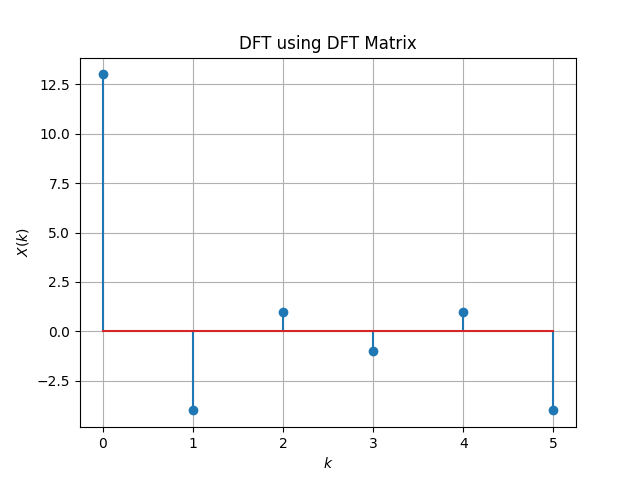
\includegraphics[width=\columnwidth]{figs/7.11.png}
		\caption{Plot of the discrete fourier transform of $\vec{x}$ using the DFT matrix}
		\label{fig-7.11}	
	\end{figure}
	
	
    \item Repeat the above exercise using the FFT
	    after zero padding $\vec{x}$.
%	    \eqref{eq:fft-mat-def}

	\solution Download the following Python code that plots Fig. 7.12
	\begin{lstlisting}
		https://github.com/shreyaswankhede12/EE3900/blob/master/Assignment%201/codes/qs%207/7.12.py
	\end{lstlisting}
	
	Run the code by executing
	\begin{lstlisting}
		python 7.12.py
	\end{lstlisting}

	\begin{figure}[!ht]
		\centering
		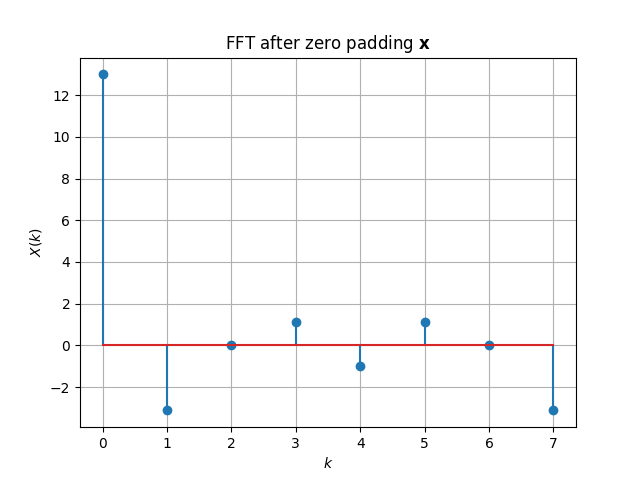
\includegraphics[width=\columnwidth]{figs/7.12.png}
		\caption{Plot of the fast fourier transform of $\vec{x}$ after zero padding}
		\label{fig-7.12}	
	\end{figure}

\item Write a C program to compute the 8-point FFT. 
	
	\solution Download the following C codes that generate the values of $X(k)$ using $8$-point FFT
	\begin{lstlisting}
		https://github.com/shreyaswankhede12/EE3900/blob/master/Assignment%201/codes/qs%207/7.13.c
	\end{lstlisting}
	
	Compile and run the C program by executing the following
	\begin{lstlisting}
		cc -lm 7.13.c
		./a.out
	\end{lstlisting}
	\item Compare and determine the running time complexities of FFT/IFFT and convolution graphically
	
	\solution Download the following C codes that measure the running times of both the algorithms
	\begin{lstlisting}
		wget https://github.com/Ankit-Saha-2003/EE3900/raw/main/Assignment_1/codes/header.h
		wget https://github.com/Ankit-Saha-2003/EE3900/raw/main/Assignment_1/codes/7.14.c
	\end{lstlisting}
	
	Compile and run the C program by executing the following
	\begin{lstlisting}
		cc -lm 7.14.c
		./a.out
	\end{lstlisting}
	
	Download the following Python code that plots Fig. 7.14 using the running times generated by the C code and fits them to appropriate functions of the input size
	\begin{lstlisting}
		https://github.com/shreyaswankhede12/EE3900/blob/master/Assignment%201/codes/qs%207/7.14.py
	\end{lstlisting}
	
	Run the code by executing
	\begin{lstlisting}
		python 7.14.py
	\end{lstlisting}

	\begin{figure}[!ht]
		\centering
		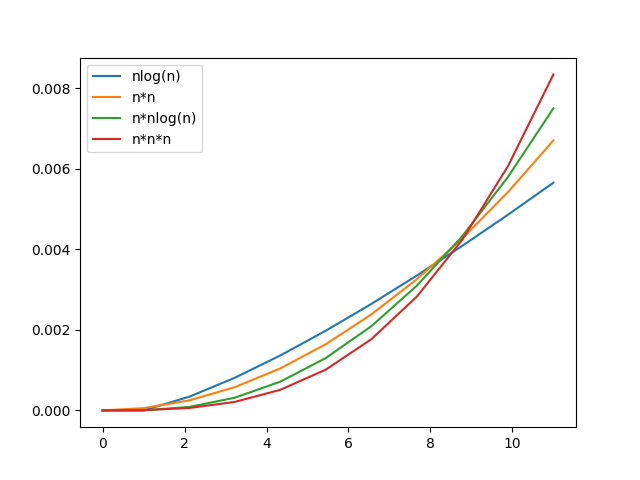
\includegraphics[width=\columnwidth]{figs/7.14.png}
		\caption{Plot of the running times of FFT/IFFT and convolution}
		\label{fig-7.14}	
	\end{figure}
	
	From the plot, it is evident that the time complexity of FFT/IFFT is $O(n \log n)$ and that of convolution is $O(n^2)$
\end{enumerate}
\section{Exercises}
\noindent Answer the following questions by looking at the python code in Problem \ref{prob:output}.
\begin{enumerate}[label=\thesection.\arabic*.,ref=\thesection.\theenumi]
\item
The command
\begin{lstlisting}
output_signal = signal.lfilter(b, a, input_signal)
\end{lstlisting}
in Problem \ref{prob:output} is executed through the following difference equation
\begin{equation}
\label{eq:iir_filter_gen}
 \sum _{m=0}^{M}a\brak{m}y\brak{n-m}=\sum _{k=0}^{N}b\brak{k}x\brak{n-k}
\end{equation}
where the input signal is $x(n)$ and the output signal is $y(n)$ with initial values all 0. Replace
\textbf{signal.filtfilt} with your own routine and verify.
\solution
Download the source code by typing the next command \\
\begin{lstlisting}
$ wget https://raw.githubusercontent.com/goats-9/ee3900-assignments/main/filter/codes/8_1.py
\end{lstlisting}
and run it using
\begin{lstlisting}
$ python3 8_1.py
\end{lstlisting}
\item Repeat all the exercises in the previous sections for the above $a$ and $b$.
\solution
For the given values, the difference equation is
\begin{align}
	&y(n) - \brak{2.52}y(n - 1) + \brak{2.56}y(n - 2) \nonumber \\
	&- \brak{1.21}y(n - 3) + \brak{0.22}y(n - 4) \nonumber \\
	&= \brak{3.45 \times 10^{-3}}x(n) + \brak{1.38 \times 10^{-2}}x(n - 1) \nonumber \\
	&+ \brak{2.07 \times 10^{-2}}x(n - 2) + \brak{1.38 \times 10^{-2}}x(n - 3) \nonumber \\
	&+ \brak{3.45 \times 10^{-3}}x(n - 4)
\end{align}
From \eqref{eq:iir_filter_gen}, we see that the transfer function can be written as follows
\begin{align}
	H(z) &= \frac{\sum_{k = 0}^{N}b(k)z^{-k}}{\sum_{k = 0}^{M}a(k)z^{-k}} \\
		 &= \sum_{i}\frac{r(i)}{1 - p(i)z^{-1}} + \sum_{j}k(j)z^{-j}
	\label{eq:trans-func}
\end{align}
where $r(i)$, $p(i)$, are called residues and poles respectively of the partial 
fraction expansion of $H(z)$. $k(i)$ are the coefficients of the direct polynomial 
terms that might be left over. We can now take the inverse $z$-transform of
\eqref{eq:trans-func} and get using \eqref{eq:anun},
\begin{align}
	h(n) &= \sum_{i}r(i)[p(i)]^nu(n) + \sum_{j}k(j)\delta(n - j)
	\label{eq:h-n-expr}
\end{align}
Substituting the values,
\begin{align}
	&h(n) = [\brak{-0.24-0.71\j}\brak{0.56+0.14\j}^n \nonumber \\
	&+ \brak{-0.24+0.71\j}\brak{0.56-0.14\j}^n \nonumber \\
	&+ \brak{-0.25+0.12\j}\brak{0.70+0.41\j}^n \nonumber \\
	&+ \brak{-0.25-0.12\j}\brak{0.70-0.41\j}^n]u(n) \nonumber \\
	&+ \brak{1.6 \times 10^{-2}}\delta(n) \\
	&\implies h(n) = \brak{1.5}\brak{0.58}^n\cos\brak{n\alpha_1 + \beta_1} \nonumber \\
	&+ \brak{0.55}\brak{0.81}^n\cos\brak{n\alpha_2 + \beta_2} \nonumber \\
	&+ \brak{1.6 \times 10^{-2}}\delta(n)
	\label{eq:h-n-real}
\end{align}
where
\begin{align}
	\tan{\alpha_1} &= 0.25 \\
	\tan{\beta_1} &= 2.96 \\
	\tan{\alpha_2} &= 0.59 \\
	\tan{\beta_2} &= -0.48
	\label{eq:h-params}
\end{align}
The values $r(i)$, $p(i)$, $k(i)$ and thus the impulse response function are computed and plotted at
\begin{lstlisting}
$ wget https://raw.githubusercontent.com/goats-9/ee3900-assignments/main/filter/codes/8_2_1.py
\end{lstlisting}
The filter frequency response is plotted at
\begin{lstlisting}
$ wget https://raw.githubusercontent.com/goats-9/ee3900-assignments/main/filter/codes/8_2_2.py
\end{lstlisting}
Observe that for a series $t_n = r^n$, $\frac{t_{n + 1}}{t_n} = r$.
By the ratio test, $t_n$ converges if $|r| < 1$. We observe that for all $i$, 
$|p(i)| < 1$ and so, as $h(n)$ is the sum of many convergent series,
we see that $h(n)$ converges and is bounded. From \eqref{eq:z_trans},
\begin{align}
	\sum_{n = 0}^{\infty}h(n) = H(1) = \frac{\sum_{k = 0}^{N}b(k)}{\sum_{k = 0}^{M}a(k)} = 1 < \infty
\end{align}
Therefore, the system is stable. From
. The following code uses the DFT matrix
to generate $y(n)$ in Fig. \eqref{fig:butter-out}.
\begin{lstlisting}
$ wget https://raw.githubusercontent.com/goats-9/ee3900-assignments/main/filter/codes/8_2_3.py
\end{lstlisting}
The codes can be run all at once by typing a small shell script
\begin{lstlisting}
$ for file in 8_2_*.py; do python ${file}; done
\end{lstlisting}
\begin{figure}[!htb]
	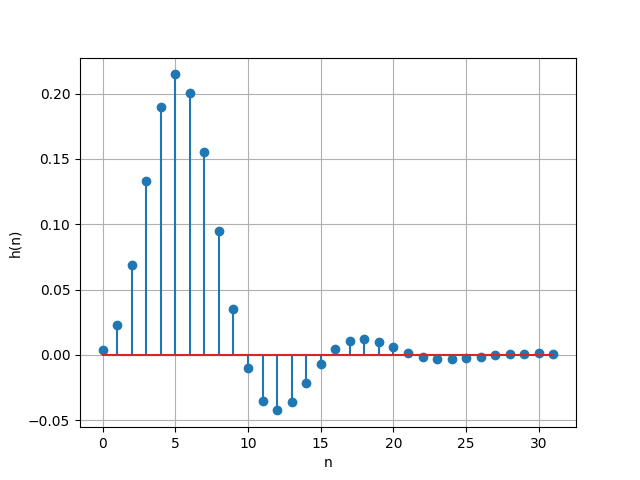
\includegraphics[width=\columnwidth]{figs/8_2_1.png}
	\caption{Plot of $h(n)$}
	\label{fig:butter-imp}
\end{figure}
\begin{figure}[!htb]
	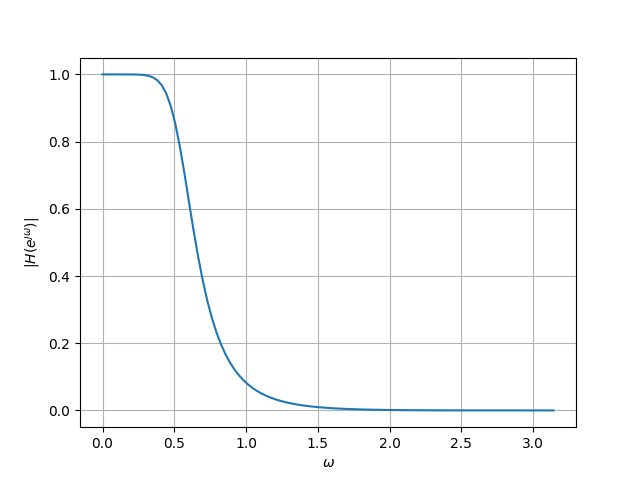
\includegraphics[width=\columnwidth]{figs/8_2_2.png}
	\caption{Filter frequency response}
	\label{fig:butter-resp}
\end{figure}
\begin{figure}[!htb]
	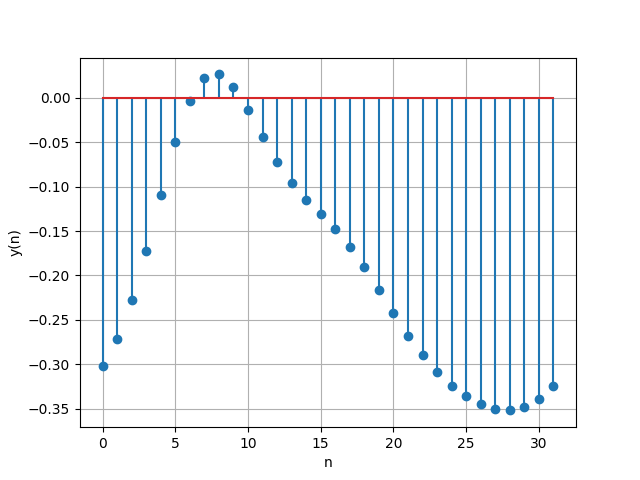
\includegraphics[width=\columnwidth]{figs/8_2_3.png}
	\caption{Plot of $y(n)$}
	\label{fig:butter-out}
\end{figure}
\item What is the sampling frequency of the input signal?
\solution
Sampling frequency $f_s = 44.1$ kHZ.
\item
What is type, order and  cutoff frequency of the above Butterworth filter?
\solution
The given Butterworth filter is low pass with order 4 and cutoff frequency 4 kHz.
\item
Modify the code with different input parameters and get the best possible output.
\solution
A better filtering was found on setting the order of the filter to be 7.
\end{enumerate}
\end{document}